\section{Functionality}
\label{sec:features}

In this section, we highlight a number of features of \oops\ that we believe
are important in an educational setting. Even though other systems may share
some of \oops' features, there is no other system that possesses all of them.

\subsection{Integrated Scripting}

In order for a theorem prover to be truly useful, it is not sufficient to be
able to answer `true' or `false' given an input formula. Rather, our
experience has shown that students will need to formulate and extend theories.
Doing this by hand by editing a single large formula quickly becomes
unmanageable.
Moreover, we want to have a powerful toolbox to assist us in the formulation
of larger theories.
This toolbox should include general programming constructs such as
loops and conditionals. Some other tools, such as the Logics Workbench, provide custom
scripting languages for this purpose. The advantage of this approach is that
the language can be tailored specifically to common usage of the prover. The
disadvantage, however, is that developing a custom language is costly.
Therefore, that the resulting language is likely to be lacking in expressive
power.
Furthermore, the user has to learn a language that has no application outside
of the prover and for which support (i.e., documentation, user community and
bug fixes) may be limited.

To address these concerns, \oops\ integrates the general-purpose scripting
language Lua.
Lua has been designed specifically to be an embeddable language and is widely
used both as an extension language and as a front-end for libraries written in
other languages.
Thus, Lua enables us to define an environment that is tailored to the needs of
theorem proving, while avoiding the concerns associated with implementing a
custom language.
See \citet{ierusalimschy2006} for a good introduction to programming in Lua.
Currently, most of \oops' functionality is available from Lua and more
extensive support is being worked on.

The above outlines our reasons for integrating \oops\ with Lua. Now
we briefly describe how \oops\ can be used through its Lua interface.
All \oops\ methods are encapsulated in the \lstinline!oops! namespace.
The basis for interaction with \oops\ through Lua is the {\em theory} concept.
A theory is, simply put, a collection of formulas. The following example code
creates a theory and adds a formula to it:
\begin{lstlisting}
th = oops.Theory()
th:add("#_1 p")
\end{lstlisting}
We define a number of operations on theories: checking of consistency,
provability of a formula within a theory and satisfiability of a formula
within a theory:
\begin{lstlisting}
print(th:consistent())           -- true
print(th:provable("#_2 #_1 p"))  -- false
print(th:satisfiable("~#_2 p"))  -- true
\end{lstlisting}
where \lstinline!--! starts a comment, here used to indicate the output
produced by the \lstinline!print! statement. 
Now, to aid in the construction of theories, we allow the explicit creation of
formulas, on which we have defined the operation of substitution. For example:
\begin{lstlisting}
th = oops.Theory()
f = oops.Formula("#_A V")
for i=1,4,1 do
        th:add(f:substitute({V = "p | q"}, {A = i}))
end
print(th)
\end{lstlisting}
which expresses that each of the agents $1, 2, 3$ and $4$ `knows' $(p \vee
q)$. The resulting output is:
\begin{lstlisting}
[#_4 (p | q), #_3 (p | q), #_1 (p | q), #_2 (p | q)]
\end{lstlisting}

This completes our description of how \oops\ is called from Lua. It must be
noted that Lua is a very powerful and complete language and that much more can be achieved than is suggested by the above examples. For
example, command-line interaction with the user is readily available through
Lua.

\subsection{Graphical User Interface}

As is discussed above, Lua provides a convenient scripting interface to \oops.
However, modern computer users do not expect to run applications from the
command-line. Even if they are used to this concept, it is not always the most
convenient method of interaction. Therefore,
\oops\ includes a very simple Graphical User Interface (GUI), in which scripts
can be displayed, edited and executed (Figure~\ref{fig:gui}). In addition,
scripts can be loaded from and saved to a file. For those who prefer to use an
external editor (e.g., there are many editors that offer syntax highlighting
for Lua), a single key combination reloads a modified file from the
file system. The application consists of two panels: the top panel shows the
current script and the bottom panel shows the
output.

\begin{figure}[p]
\centering
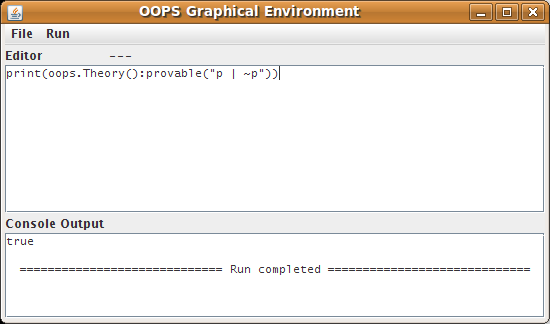
\includegraphics[scale=.50]{images/gui}
\caption{The \oops\ Graphical User Interface.}
\label{fig:gui}
\end{figure}

Though minimal, the GUI greatly enhances the convenience with which \oops\ can
be used. Firstly, script and output are shown in one place, allowing for easy
cross-referencing. Second, scripts are run through a single key combination
(or invocation from the menu). Finally, the load, save and refresh functionalities
give the user the freedom to use the integrated editor or an external editor
of choice with equal convenience.

\subsection{Free and Convenient Distribution}

As we noted in Section~\ref{sec:introduction}, most current proof tools have
problems related to either platform dependence, aging dependencies, lack of
maintenance or difficult installation procedures. \oops\ addresses these
problems in several ways.
First, \oops\ is implemented in pure Java, which means that \oops\ will run on
any operating system for which a Java virtual machine is available. This is
true for most operating systems available today.
Second, \oops\ is distributed as a ZIP file that includes all dependencies.
No installation is needed, one simply extracts the ZIP file and double-clicks
the resulting {\texttt oops.jar} file.
Hence, \oops\ is platform independent and easy to run, having no dependencies
apart from the Java VM and what is provided in the \oops\ distribution.

The concern of continued maintenance is harder to address. To ensure that
\oops\ can be used and extended in the future by anyone who wishes to do so,
we provide the full source code\footnote{http://github.com/gertvv/oops} under
the GNU General Public License (GPL). It is our hope that others will
contribute extensions to \oops.

\subsection{Visualization of Tableaux}

When a student is learning to work with modal logics, a prover can often give surprising
results. He or she may encounter undesirable outcomes when constructing a
theory and would like to be able to `debug' the theory by inspecting the proof
process. Moreover, inspecting generated tableaux may enhance understanding of
tableau methods and the semantics of modal logics in general.
To support this, \oops\ includes a visualization module for labeled tableaux.
Figure~\ref{fig:tableauVis} shows an example of such a visualization. 
The tableau is drawn as a tree.
In the tree, nodes are numbered  in the order in which they are added
(left-most on each line).
After the node number, the
label is shown, followed by the formula. Finally, the rule that resulted in
the creation of the specific node and the node number to which the rule
matched are given.

\begin{figure}[p]
\centering
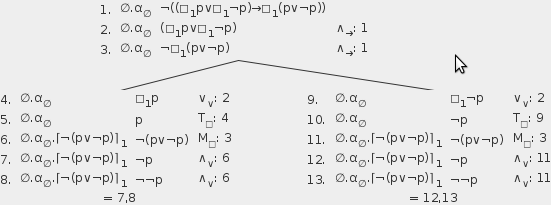
\includegraphics[scale=.50]{images/tableauVis}
\caption{Visualization of the tableau that checks provability of $\varphi$, by
attempting to satisfy $\neg \varphi$, where
$\varphi = ((\square_1 p \vee \square_1 \neg p) \to \square_1(p \vee \neg p))$.
In this case, the tableau is closed (i.e. $\varphi$ is provable), as indicated
by the $= (m, n)$ under each branch, where $m$ and $n$ indicate the line
numbers at which two contradicting formulas are found.}
\label{fig:tableauVis}
\end{figure}

\begin{figure}[p]
\centering
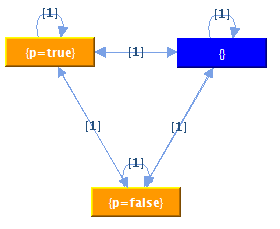
\includegraphics[scale=.50]{images/modelVis}
\caption{Visualization of a counter-model for $\varphi = (\Box_1 p \vee \Box_1
\neg p)$. The `main' world is indicated in blue.}
\label{fig:modelVis}
\end{figure}

The visualization is implemented as an observer on the tableau generator
(see Section~\ref{sec:implementation}).
The Lua code to generate
Figure~\ref{fig:tableauVis} is as follows (note that the command-line output
will be \lstinline!true!):
\begin{lstlisting}
oops.attachTableauVisualizer()
print(oops.Theory():provable(
	"(#_1 p | #_1 ~p) > #_1(p | ~p)"))
\end{lstlisting}

\subsection{Visualization of Countermodels}

In addition to being able to view the tableau, it may be helpful to be able to
inspect a model that the tableau corresponds to.
In case the tableau is open, the generated model will generally be more
insightful, as it does not contain any redundant information.
As is the case for tableau visualization, visualization of (counter-)models may
enhance understanding of the semantics of modal logics.



Figure~\ref{fig:modelVis} is generated by the following Lua code (note that
the command-line output will be \lstinline!false!):
\begin{lstlisting}
oops.attachModelConstructor()
print(oops.Theory():provable("#_1 p | #_1 ~p"))
oops.showModel() 
\end{lstlisting}
As the reader will notice, the invocation of the model visualization is done
differently from the tableau visualization.
This is because we treat models as entities in their own right.
In fact, the call \lstinline!oops.getModel()!  can be used to retrieve the most
recently constructed model, if the last invocation of the tableau generator
resulted in an open tableau.
The Lua \lstinline!print! function will output a textual representation of the
model.
However, further programmatic manipulation and inspection of models is future
work.
